\chapter{ Network Aware Predictive Pre-Loading }

Lazy loading modules in Angular, allows for javascript loading to be optimized. 
That is, so browser only loads the page the user is navigating to. This helps to
decrease the initial load time. However, depending on how expensive including a
module is, pre-loading can save you time. Pre-loading is a strategy that allows
for modules in Angular to be loaded as soon as possible. Modules can be pre-loaded 
either all at the same time, or a select few, or when a custom event happens. You
can check yourself how long it takes for a module to load, and the potential value 
of pre-loading. Open up your developer console tool(I'm using Chrome), navigate to
the js section, of the network tab, and then load the page you want to test. 

\begin{figure}[h]
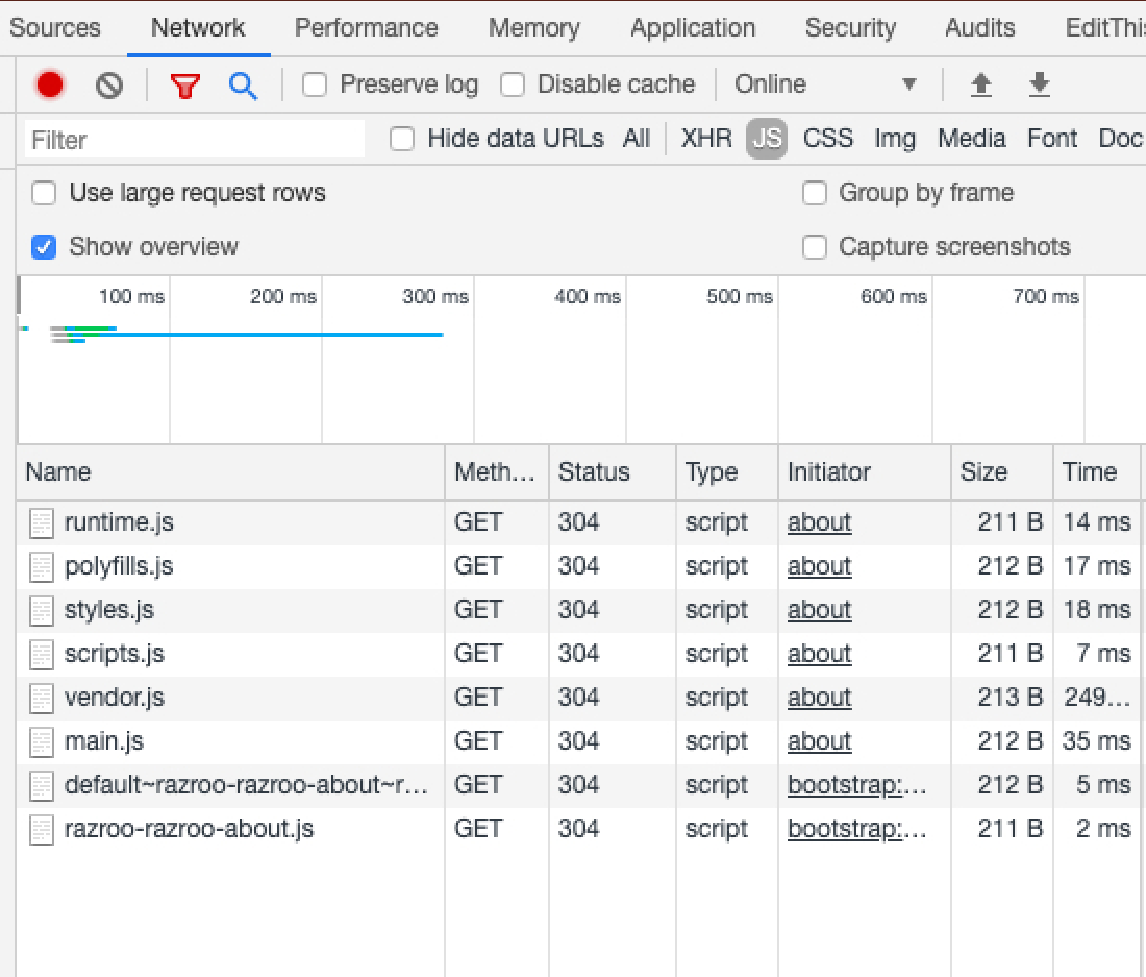
\includegraphics[width=414pt]{architecture/lazy-loading/network-aware-preloading/network-preloading-console-screenshot.pdf}
\caption{As we can see, it took 2ms to download the Razroo About page.}
\end{figure}

\section{ Being Aware of How Much Time Pre-Loading Saves }
You might be curious as to how much time is actually saved with regards to 
pre-loading? I was curious as well. I tried personally(as shared in the screenshot 
above), and the amount of time saved, to be honest, is negligable. However, I also
realize that the app I am working on has a minimal amount of modules. I can see that 
for another app, wherein there are multiple modules that are loaded. Therefore, 
let's throw out an arbitrary number. If you have a module that is going to 
use more than 20 imports inside of it's module, then worry about a pre-loading 
strategy. Regardless, it is something to be aware of, and here is how to go 
around implementing pre-loading. 

\section{Pre-Load Everything}
While this strategy will rarely work for any real-world application, there is 
an option to pre-load every module in Angular. To do so, you would use \lstinline{PreloadAllModules}
as your preloading strategy: 
\begin{lstlisting}
import { RouterModule, PreloadAllModules } from '@angular/router';

@NgModule({
  imports: [
    RouterModule.forRoot(routes, {
      preloadingStrategy: PreloadAllModules,
    }),
  ],
})
class AppRoutingModule {}
\end{lstlisting}

\section{ Custom Pre-Loading }
What does make more sense in an enterprise setting, is custom pre-loading
modules. That is, pre-load the more expensive modules, and do not pre-load those
that are less expensive. In addition, make the pre-loading happen at a time more 
convenient for the app. Let's dive into what that means and how we can do that.

Angular offers the ability to pre-load specific modules(as opposed to all of them 
at the same time, as we showed before). It offers a \lstinline{preload}
method that takes two arguments: 
\begin{enumerate}
  \item route - Route object to tap into, for the load function.
  \item load - Function that when run, triggers the module being loaded
\end{enumerate}

\subsection{General Strategy}
If we wanted to pre-load some modules, and did not want to pre-load others, we
would follow the following strategy:
\begin{enumerate}
  \item Give our route unique data(i.e. \lstinline{preload: true})
   to be used within our custom pre-loading function.
  \item Create a custom pre-loading function, that makes use of our unique data. 
  \item Pass in custom pre-loading as a provider to the \lstinline{preloadingStrategy} 
  key.
\end{enumerate}

\subsection{Strategy Exemplified in Code}
\subsubsection{Give Route Unique Data}
\begin{lstlisting}[caption=app.routing.module.ts]
import { NgModule } from '@angular/core';
import { RouterModule } from '@angular/router';

@NgModule({
  imports: [
    RouterModule.forRoot(
      [
        {
          path: 'books',
          loadChildren: () =>
            import('@razroo/razroo/books').then(
              module => module.RazrooBooksModule
            ),
          data: { preload: true }
        },
        {
          path: 'consulting',
          loadChildren: () =>
            import('@razroo/razroo/consulting').then(
              module => module.RazrooConsultingModule
            )
        },
      ],
      {
        initialNavigation: 'enabled',
        relativeLinkResolution: 'corrected'
      }
    )
  ],
  exports: [RouterModule]
})
export class RazrooAppRoutingModule {}
\end{lstlisting}

\subsubsection{Custom Function For Pre-Loading}
\begin{lstlisting}[caption=custom-preloading.ts]
export class PreloadSelectedModulesList implements PreloadingStrategy {
  preload(route: Route, load: Function): Observable<any> {
    return route.data && route.data.preload ? load() : of(null);
  }
}
\end{lstlisting}

\textit{It is worthwhile to note that Razroo put's the \lstinline{custom-preloading.ts} 
util file in the \lstinline{libs/common/services} folder.}

\subsubsection{Pass in custom pre-loading as a Provider}
\begin{lstlisting}[caption=app.routing.module.ts]
import { NgModule } from '@angular/core';
import { RouterModule } from '@angular/router';
import { PreloadSelectedModulesList } from '@razroo/common/ui/utils';

@NgModule({
  imports: [
    RouterModule.forRoot(
      [
        // ...routes go here
      ],
      {
        preloadingStrategy: PreloadSelectedModulesList
        //...
      }
    )
  ],
  exports: [RouterModule]
})
export class RazrooAppRoutingModule {}
\end{lstlisting}

\subsection{ How to See That Module Has Indeed Pre-Loaded }
In order to see that your module has pre-loaded, you can go to the JS
tab in your chrome dev tools. There you will see the amount of time it 
took to load. For me personally, it took about 4 ms. So that is the amount 
of time you might be saving for smaller modules. I would imagine that 
larger modules would take longer. 

\section{ Enabling Module Pre-loading on Custom Event }
If we would like to extend the pre-loading architecture one step further, 
tying in custom events with custom pre-loading, will make things even 
more efficient. In particular, when a user hovers over a navigation menu item, 
we can pre-load a module. 

\subsection{ General Strategy }
The general strategy will look somewhat similar custom pre-loading. 
With some modified/added steps.

\begin{enumerate}
  \item Give our route some unique data(i.e. preload: true)
   to be used within our custom-preloading function.
   \item Create a separate service that will be used to trigger a next on the 
   observable contained in the custom-preloading function. 
   \item Create custom pre-loading function, that makes use of our unique data. In addition, 
   give it access to a \lstinline{Subject}, so it can be triggerred, by an outside service. 
   \item Pass in custom pre-loading service as a provider to the \lstinline{preloadingStrategy} 
   key.
  \item Use a mouseover function, that can trigger the service.
\end{enumerate}

\subsection{ Strategy Exemplified in Code }
We will be giving our route the same unique data: 

\subsubsection{Give Route Unique Data}
\begin{lstlisting}[caption=app.routing.module.ts]
import { NgModule } from '@angular/core';
import { RouterModule } from '@angular/router';

@NgModule({
  imports: [
    RouterModule.forRoot(
      [
        {
          path: 'books',
          loadChildren: () =>
            import('@razroo/razroo/books').then(
              module => module.RazrooBooksModule
            ),
          data: { preload: true }
        },
        {
          path: 'consulting',
          loadChildren: () =>
            import('@razroo/razroo/consulting').then(
              module => module.RazrooConsultingModule
            )
        },
      ],
      {
        initialNavigation: 'enabled',
        relativeLinkResolution: 'corrected'
      }
    )
  ],
  exports: [RouterModule]
})
export class RazrooAppRoutingModule {}
\end{lstlisting}

\subsubsection{ Create a Separate Service to Trigger Pre-Loading }
We will be creating a separate service, that will be used within our CustomPreloadingService
to trigger 


\subsubsection{Custom Pre-Loading Service}
\begin{lstlisting}
import { Injectable } from '@angular/core';
import { PreloadingStrategy, Route } from '@angular/router';
import { EMPTY, Observable, of } from 'rxjs';
import { mergeMap } from 'rxjs/operators';
import { OnDemandPreloadOptions, OnDemandPreloadService } from './on-demand-preload.service';

@Injectable({ providedIn: 'root', deps: [OnDemandPreloadService] })
export class OnDemandPreloadStrategy implements PreloadingStrategy {
  private preloadOnDemand$: Observable<OnDemandPreloadOptions>;

  constructor(private preloadOnDemandService: OnDemandPreloadService) {
    this.preloadOnDemand$ = this.preloadOnDemandService.state;
  }

  preload(route: Route, load: () => Observable<any>): Observable<any> {
    return this.preloadOnDemand$.pipe(
      mergeMap(preloadOptions => {
        const shouldPreload = this.preloadCheck(route, preloadOptions);
        return shouldPreload ? load() : EMPTY;
      })
    );
  }

  private preloadCheck(route: Route, preloadOptions: OnDemandPreloadOptions) {
    return (
      route.data &&
      route.data['preload'] &&
      [route.path, '*'].includes(preloadOptions.routePath) &&
      preloadOptions.preload
    );
  }
}
\end{lstlisting}

\subsubsection{Pass in Custom Pre-loading Service as a Provider}
\begin{lstlisting}[caption=app.routing.module.ts]
import { NgModule } from '@angular/core';
import { RouterModule } from '@angular/router';
import { CustomPreloadingService } from '@razroo/common/services';

@NgModule({
  imports: [
    RouterModule.forRoot(
      [
        // ...routes go here
      ],
      {
        preloadingStrategy: CustomPreloadingService
        //...
      }
    )
  ],
  exports: [RouterModule]
})
export class RazrooAppRoutingModule {}
\end{lstlisting}

\subsubsection{Trigger Service}
In our particular scenario, as would make sense for alot of applications, is trigger 
module pre-loading on mouseover. We can therefore do something such as the following: 
\begin{lstlisting}
<a
  [routerLink]="item.link"
  class="nav-link"
  (mouseover)="preloadBundle('heroes')"
  >heroes</a
>  
\end{lstlisting}

\begin{lstlisting}
preloadBundle(routePath) {
  this.preloadOnDemandService.startPreload(routePath);
}
\end{lstlisting}

\section{Creating a Directive}
Using this method, we can also create a directive to allow the logic for 
preloading to be re-usable. 

\begin{lstlisting}[caption=preload.directive.ts]
import { Directive, ElementRef, HostListener } from '@angular/core';
import { OnDemandPreloadService } from '@razroo/common/services';

@Directive({
  selector: '[razrooPreload]'
})
export class PreloadDirective {

  constructor(private elementRef : ElementRef,
              private onDemandPreloadService: OnDemandPreloadService) {}

  @HostListener('mouseenter')
  onMouseEnter() {
    const pathName = this.elementRef.nativeElement.attributes.routerlink.value;
    this.onDemandPreloadService.startPreload(pathName);
  }
}
\end{lstlisting}

In the above code for the directive we are assuming that there 
is a routerlink, on the a tag we are looking for. If there isn't, the directive 
will return an error. This allows us to now simply add the following: 
\begin{lstlisting}
  <a routerLink="books" razrooPreload>
  </a> 
\end{lstlisting}

When the user mouses over, we will now be able to see in our chrome console,
that the appropriate module has been pre-loaded. 

\section{ Network Aware Pre-Loading }
We've created an on-demand pre-loading strategy. When a user hovers over a 
menu item, and before they click on it, it will already begin to pre-load. 
It's a very clever strategy, that uses the user's own intent to maximize 
the app's performance. However, let's say in our pre-loading strategy, we 
have three pages. 
\begin{enumerate}
  \item About 
  \item Product
  \item Application Page
\end{enumerate}

The application page opens up a very heavy js bundle, that take's about 
.25 seconds to load on a fast network. However, on a slower network it might 
take around an entire second. In such a slow netowrk, if the user hovers
over the large applications page first, and then the much smaller about page,
our pre-loading strategy might have the reverse effect in such a slow network.
If we want an air tight strategy that takes care of all scenarios, it makes 
sense for us to go ahead and take network connection into account. 

\subsection{Network Information API}
I have seen some blogs in this regards suggesting use of the network
information api, for figuring out the speed of the network. It's actually 
interesting, W3C specs have included talks for the Network Information API 
since \href{https://www.w3.org/TR/2011/WD-netinfo-api-20110607/}{2011}. However, 
there have been many discussions since then, landing on the latest version
solidified in \href{https://www.w3.org/TR/netinfo-api/}{2014}. 

First and foremost, before discussing how to use this API, it probably makes 
sense to go ahead and discuss that for the API we plan on using, current usage 
is at about 70\%. It's worth noting that the lions share of the percentage is 
with regards to IOS Safari(a whopping 10\%), which does not support this feature. 
In addition, Firefox currently does not support. However, Chrome which is used 
by the majority of users between Android and Desktop is at about 60\% on it's own. 

Still the API has ways to go, so understandably, this is not a fool proof 
solution. However, seeing as support is somewhat decent, and this is relatively 
easy to implement, let's go ahead and do so. 

\subsection{ Strategy Exemplified in Code }

First and foremost, since the Network Information API, is still experiemental 
technology, Typescript will not support it as part of it's core library yet. 
Howeever, the following \href{https://github.com/lacolaco/network-information-types}{types}
is complete in my opinion, and no reason to add anything special. 

\begin{lstlisting}[caption=custom-preloading.ts]
hasGoodConnection(): boolean {
  const conn = navigator.connection;
  if (conn) {
    if (conn.saveData) {
      return false; // save data mode is enabled, so dont preload
    }
    const avoidTheseConnections = ['slow-2g', '2g'];
    // 'slow-2g', '2g', '3g', or '4g'
    const effectiveType = conn.effectiveType || '';
    if (avoidTheseConnections.includes(effectiveType)) {
      return false;
    }
  }
  return true;
}
\end{lstlisting}

In the above function, we are using the navigator.connection effective types, 
which tells us the connection that the user is currently experiencing. If it is slow-2g, 
or 2g, we return false in this function. We can now hook it up into the pre-emptive loading
code we had before. 

Because the network information api is experimental technology, let's just add a custom 
type declaration in our file, to knock out any type errors that we receive. Putting it 
all together, our file will something like the following: 
\begin{lstlisting}[caption=custom-preloading.service.ts]
import { Injectable } from '@angular/core';
import { PreloadingStrategy, Route } from '@angular/router';
import { EMPTY, Observable, of } from 'rxjs';
import { mergeMap } from 'rxjs/operators';
import { OnDemandPreloadOptions, OnDemandPreloadService } from './on-demand-preload.service';
export declare var navigator;

@Injectable({ providedIn: 'root', deps: [OnDemandPreloadService] })
export class CustomPreloadingService implements PreloadingStrategy {
  private preloadOnDemand$: Observable<OnDemandPreloadOptions>;

  constructor(private preloadOnDemandService: OnDemandPreloadService) {
    this.preloadOnDemand$ = this.preloadOnDemandService.state;
  }

  preload(route: Route, load: () => Observable<any>): Observable<any> {
    return this.preloadOnDemand$.pipe(
      mergeMap(preloadOptions => {
        const shouldPreload = this.preloadCheck(route, preloadOptions);
        const hasGoodConnection = this.hasGoodConnection();
        if(shouldPreload && hasGoodConnection) {
          return load();
        }
        else {
          return EMPTY;
        }
      })
    );
  }

  private preloadCheck(route: Route, preloadOptions: OnDemandPreloadOptions) {
    return (
      route.data &&
      route.data['preload'] &&
      [route.path, '*'].includes(preloadOptions.routePath) &&
      preloadOptions.preload
    );
  }

  private hasGoodConnection(): boolean {
    const conn = navigator.connection;
    if (conn) {
      if (conn.saveData) {
        return false; // save data mode is enabled, so dont preload
      }
      const avoidTheseConnections = ['slow-2g', '2g'];
      // 'slow-2g', '2g', '3g', or '4g'
      const effectiveType = conn.effectiveType || '';
      if (avoidTheseConnections.includes(effectiveType)) {
        return false;
      }
    }
    return true;
  }
}
\end{lstlisting}

If you would like to try it yourself, throttle the network speed using the console 
and see that it doesn't download. 